% !TEX encoding = UTF-8
% !TEX TS-program = pdflatex
% !TEX root = ../tesi.tex

%**************************************************************
\chapter{Progettazione} %TODO e codifica
\label{cap:progettazione}
%**************************************************************

\intro{Il capitolo corrente ha lo scopo di illustrare l'architettura del plugin nel  dettaglio con il supporto di diagrammi e le scelte progettuali effettuate.}\\

%**************************************************************
\section{Tecnologie}
\label{sec:tecnologie-strumenti}

In questa sezione viene data una panoramica delle tecnologie e librerie principali utilizzate.

\subsection*{JavaX}
\begin{itemize}
    \item javax.annotation (per le annotazioni Nonnull e Nullable)
    \item javax.ws.rs.core (per la creazione di risorse: Low-level interfaces and annotations used to create RESTful service resources.)
    \item javax.xml.bind.annotation (per la trasformazione di JSON in oggetti Java)
\end{itemize}


\subsection*{Codehaus Plexus}
Codehaus Plexus è una collezione di componenti usata da Apache Maven.
Per ZipArchiver e utilità.
\begin{itemize}
    \item org.codehaus.plexus.archiver
    \item org.codehaus.plexus.util
\end{itemize}

\subsection*{Maven}
\begin{itemize}
    \item org.apache.maven.plugins.annotations (Mojo, Paremeter, ecc)
    \item org.apache.maven.plugin (Exceptions)
\end{itemize}

\subsection*{Jersey}
Per il client.


%**************************************************************
\section{Diagramma dei package} %TODO da rifare
\label{sec:diagramma-package}
\begin{figure}[H]
    \centering
    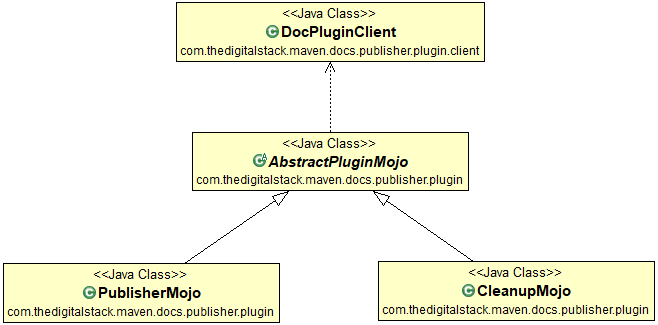
\includegraphics[width=0.9\textwidth]{immagini/PackageDiagram.png}\\
    \caption{Diagramma dei package}
\end{figure}

%**************************************************************
\section{Diagramma delle classi}
\label{sec:diagramma-classi}
\begin{figure}[H]
    \centering
    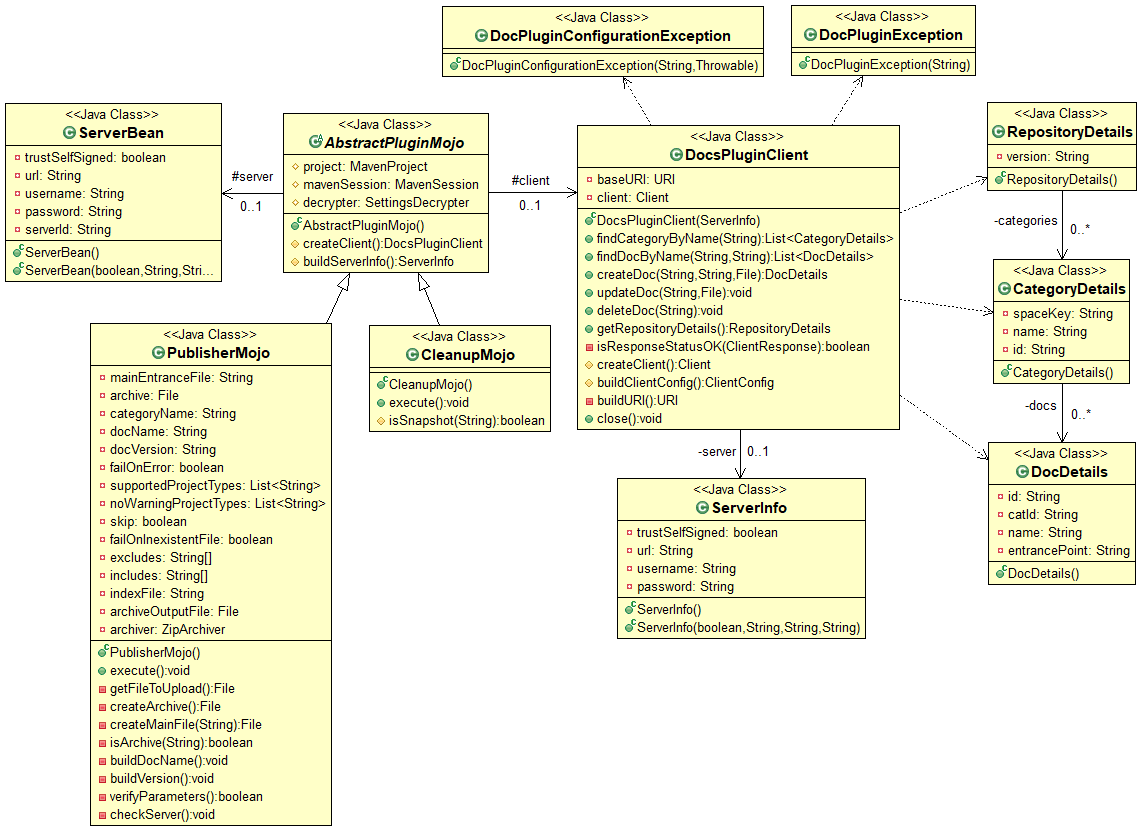
\includegraphics[width=\textwidth]{immagini/ClassD.png}\\
    \caption{Diagramma delle classi}
\end{figure}


%**************************************************************
% \section{Ciclo di vita del software}
% \label{sec:ciclo-vita-software}

%**************************************************************
% \section{Progettazione}
% \label{sec:progettazione}

% \subsubsection{Namespace 1} %**************************
% Descrizione namespace 1.

% \begin{namespacedesc}
%     \classdesc{Classe 1}{Descrizione classe 1}
%     \classdesc{Classe 2}{Descrizione classe 2}
% \end{namespacedesc}


%**************************************************************
\section{Design Pattern utilizzati}

%**************************************************************
% \section{Codifica}
